\section{Experiments}

\textbf{CVPPP leaf segmentation}. One instance segmentation benchmark is the
CVPPP plant leaf dataset \cite{minervini14cvppp}, which was developed due to
the importance of instance segmentation in plant phenotyping. We ran the A1
subset of CVPPP plant leaf segmentation dataset. We trained our model on 128
labelled images, and report results on the 33 test images. We compare our
performance to \cite{romeraparedes15ris}, and other top approaches that were
published with the CVPPP conference; See the collation study
\cite{scharr16leaf} for details of these  other approaches.

\textbf{KITTI car segmentation}. Instance segmentation also provides rich
information in the context of autonomous driving. Following
\cite{zhang15insseg, zhang16insseg, uhrig16insseg}, we also evaluated the model
performance on KITTI car segmentation dataset. We trained the model with 3712
training images, and report performance on 144 test images. We also examine the
relative importance of model components via ablation studies.

\textbf{MS-COCO counting}. Additionally, we train class specific models on
MS-COCO and test counting performance on the results. We chose ``person'' and
``zebra'' because these are the two of the most common classes in VQA
questions. We report counting performance on images with at least one instance
of the class: 677 zebra images, and 21634 ``person'' images.

\begin{table}
\begin{minipage}[t]{.48\textwidth}
% \begin{minipage}[t]{1.0\textwidth}
\caption{Leaf segmentation and counting performance}
\label{tab:cvppp}
\centering
\begin{small}

% \resizebox{1.0\columnwidth}{!}{
\begin{tabular}{l|ll}
\toprule
\toprule
                                  & \*{SBD} \u     & \*{|DiC|} \d    \\
\midrule
RIS+CRF \cite{romeraparedes15ris} & 66.6 (8.7)     & 1.1 (0.9)       \\
MSU \cite{scharr16leaf}           & 66.7 (7.6)     & 2.3 (1.6)       \\
Nottingham \cite{scharr16leaf}    & 68.3 (6.3)     & 3.8 (2.0)       \\
Wageningen \cite{yin14leaf}       & 71.1 (6.2)     & 2.2 (1.6)       \\
IPK \cite{pape14ipk}              & 74.4 (4.3)     & 2.6 (1.8)       \\
PRIAn \cite{giuffrida15count}     & -              & 1.3(1.2)        \\
\midrule
Ours (FCN + Canvas)               & 79.3 (9.2)     & 0.9 (1.0)       \\
Ours (FCN + ConvLSTM)             & 80.4 (8.9)     & 1.0 (0.8)       \\
Ours (Canvas)                     & \*{84.9} (4.8) & \*{0.8} (1.0)   \\
\bottomrule
\end{tabular}
% }
\end{small}
% \end{table}
% }
\end{minipage}
\qquad
\begin{minipage}[t]{.48\textwidth}
\label{tab:vqa}
\caption{Counting performance on MS-COCO}
\centering
\begin{small}
\begin{tabular}{l|lll}
\toprule
\toprule
                                     & \*{Category} & \*{MWCov} \u  & \*{|DiC|} \d \\
\midrule
detect \cite{chattopadhyay16count}   & Person       & -             & 3.22     \\
aso-sub \cite{chattopadhyay16count}  & Person       & -             & \*{1.36} \\
\midrule
Ours                                 & Person       & 48.3          & 2.09     \\
\midrule
\midrule
detect \cite{chattopadhyay16count}   & Zebra        & -             & 2.56     \\
aso-sub \cite{chattopadhyay16count}  & Zebra        & -             & 1.03     \\
\midrule
Ours                                 & Zebra        & 65.3          & \*{0.85} \\
\bottomrule
\end{tabular}
\end{small}
\end{minipage}
\end{table}

\newcommand{\cvpppImg}[1] {
\includegraphics[width=0.133\textwidth]{./figs/cvppp_img/plant#1_rgb.png} &
\includegraphics[width=0.133\textwidth]{./figs/cvppp_gt/plant#1_label.png} &
\includegraphics[width=0.133\textwidth]{./figs/cvppp_out/plant#1_label.png}}

\begin{figure}
\centering
\begin{small}
\resizebox{\columnwidth}{!}{
\begin{tabular}{ccccccc}
Image & GT & Ours & & Image & GT & Ours \\
\cvpppImg{029} & & \cvpppImg{137}\\
\\
\cvpppImg{042} & & \cvpppImg{119}
\end{tabular}
}
\caption{Examples of our instance segmentation output on CVPPP leaf dataset.
In this paper, instance colors are determined by the order of the model output
sequence.}
\label{fig:cvppp_out}
\end{small}
\end{figure}

\begin{table}[t]
\caption{KITTI vehicle segmentation results}
\label{tab:kitti}
\centering
\begin{small}
\begin{tabular}{l|llllll}
\toprule
\toprule
                                 & \*{FG IoU} \u & \*{MWCov} \u & \*{MUCov} \u & \*{AvgFP} \d & \*{AvgFN} \d \\
\midrule
No Sched. Samp.                  & 87.6          & 78.1         & 62.9         & 0.139        & 0.361        \\
No Post Proc.                    & 83.0          & 78.7         & 65.8         & 0.222        & 0.431        \\
\midrule    
DenseCRFv1 \cite{zhang15insseg}  & 77.3          & 70.9         & 52.2         & 0.597        & 0.736        \\
DenseCRFv2 \cite{zhang16insseg}  & 78.5          & 74.1         & 55.2         & 0.417        & 0.833        \\
FCN+Depth \cite{uhrig16insseg}   & 84.1          & 79.7         & \*{75.8}     & 0.201        & \*{0.159}    \\
\midrule
Ours (Canvas)                    & 86.9          & 72.2         & 59.4         & \*{0.090}    & 0.438        \\
Ours (FCN + Canvas)              & \*{86.8}      & 81.0         & 66.6         & 0.167        & 0.396        \\
Ours (FCN + ConvLSTM)            & \*{86.8}      & \*{82.2}     & 67.7         & 0.188        & 0.382        \\
\bottomrule
\end{tabular}
\end{small}
\end{table}

\newcommand{\kittiImg}[1] {
\includegraphics[width=0.3\textwidth]{./figs/kitti_img/#1.png} &
\includegraphics[width=0.3\textwidth]{./figs/kitti_gt/#1.png} &
\includegraphics[width=0.3\textwidth]{./figs/kitti_out/#1.png}}

\begin{figure}
\centering
\begin{small}
\resizebox{\columnwidth}{!}{
\begin{tabular}{ccc}
Image & GT & Ours \\
\kittiImg{002142} \\
\\
\kittiImg{001415} \\
\\
\kittiImg{005057} \\
\\
\kittiImg{004369} \\
\end{tabular}
}
\caption{Examples of our instance segmentation output on KITTI}
\label{fig:kitti_out}
\end{small}
\end{figure}

\begin{figure}[h]
% \begin{wrapfigure}{rt}{0.5\textwidth}
\centering
% \resizebox{0.45\textwidth}{!}{
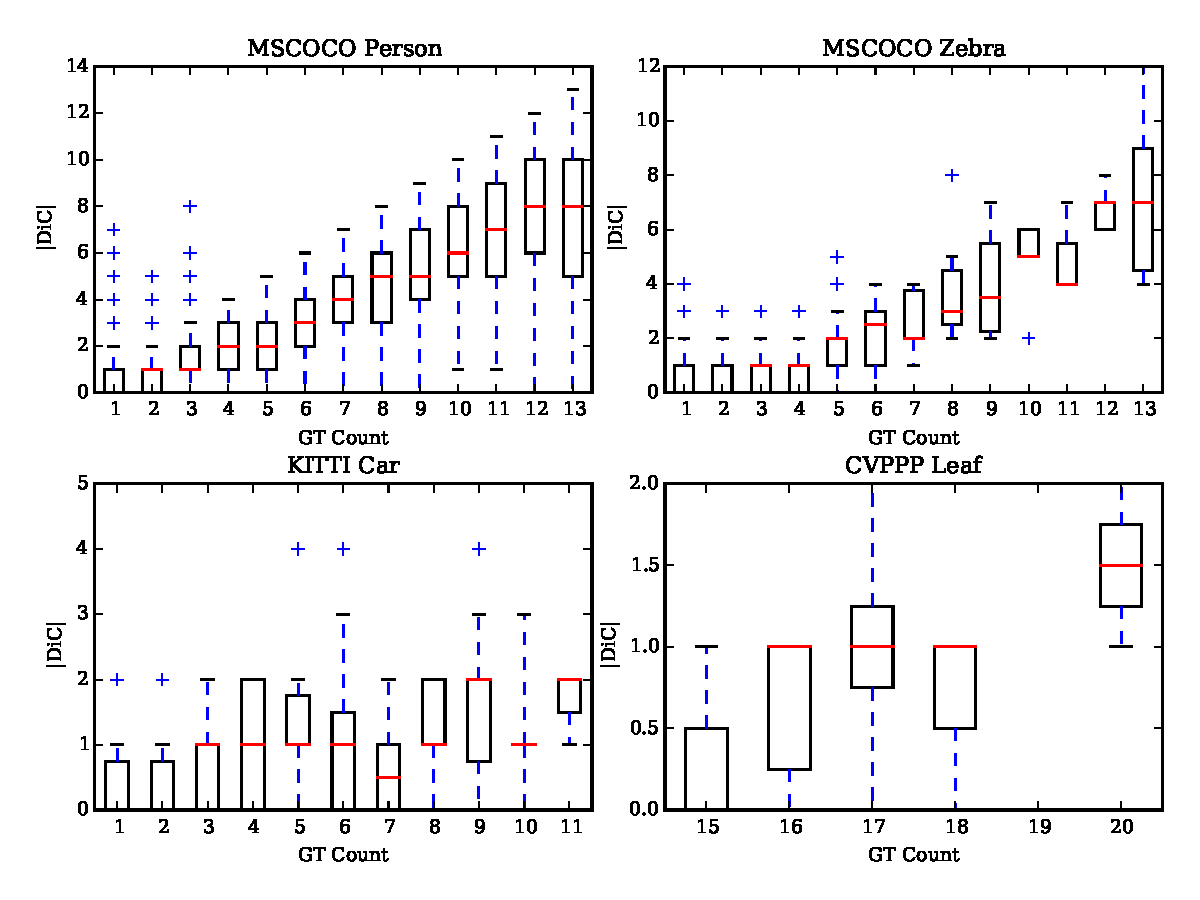
\includegraphics[width=0.8\textwidth]{count.pdf}
\caption{Absolute difference in count between the model and ground-truth as 
a function of the number of objects, in the various datasets.}
\label{fig:count}
% }
% \end{wrapfigure}
\end{figure}


\textbf{Evaluation metrics}. We report the  metrics used by the other studies
in the respective benchmarks: symmetric best dice (SBD) for leaf segmentation
(See Equation~\ref{eq:bd}, \ref{eq:sbd}) and mean (weighted) coverage (MWCov,
MUCov) for car segmentation (See Equation~\ref{eq:mwcov}, \ref{eq:mucov}). Both
coverage score measures the instance-wise IoU for each ground-truth instance
averaged over the image. MWCov further weights the score by the size of the
ground-truth instance segmentation (larger object gets larger weight).
\vspace{-3pt}
\begin{align}
\label{eq:bd}
\text{DICE}(A, B) &= \frac{2 |A \cup B|}{|A| + |B|} \ \ \ \ \ \ \ \
\text{BD}(\{A_i\}, B) = \max_{i} \text{DICE}(A_i, B) \\
\label{eq:sbd}
\text{SBD}(\{\hat{y}_i\}, \{y_j\}) &= 
\min \left(\frac{1}{N} \sum_j \text{BD}(\{\hat{y}_i\}, y_j), \frac{1}{N}
\sum_i \text{BD}(\hat{y}_i, \{y_j\}) \right)
\end{align}
\vspace{-12pt}
\begin{align}
\label{eq:mwcov}
\text{MWCov}(\{y_i\}, \{y_j^*\}) &= \frac{1}{N} \sum_i 
\frac{|y_i|}{\sum_i |y_i|} \max_j
\text{IoU}(y_i, y_j^*)\\
\label{eq:mucov}
\text{MUCov}(\{y_i\}, \{y_j^*\}) &= \frac{1}{N} \sum_i 
\max_j \text{IoU}(y_i, y_j^*)
\end{align}

Counting is measured in absolute difference in count (|DiC|) (See
Equation~\ref{eq:dic}), average false positive (AvgFP), and average false
negative (AvgFN). False positive is the number of predicted instances that do
not overlap with the ground-truth, and false negative is the number of ground-
truth instances that do not overlap with the prediction.
\vspace{-3pt}
\begin{align}
\label{eq:dic}
|DiC| = \frac{1}{N}\sum_i |count_i - count_i^*|
\end{align}
\vspace{-12pt}

\subsection{Results \& discussion}
\vspace{-3pt}
In the leaf segmentation task, our best model outperforms the previous 
state-of-the-art by a large margin in both segmentation and counting.
Table~\ref{tab:cvppp} shows that the models with FCN overfit and 
scores lower than the simpler version. This is sensible as the dataset size
is small, and including the FCN significantly increases the input dimension and
number of parameters.

In the car segmentation task, our model achieves the state-of-the-art MWCov
shown in Table~\ref{tab:kitti}, but our MUCov is lower than results reported by
Uhrig et al. \cite{uhrig16insseg}. One possible explanation is their inclusion
of depth information during training, which may help the model disambiguate
distant object boundaries. Moreover, their bottom-up ``instance fusion'' method
plays a crucial role (omitting this leads to a steep performance drop); this
likely helps segment smaller objects, whereas our box network does not reliably
detect distant cars.

In the zebra counting task, we found that our model outperforms the detector
and NMS method, and associative-subitizing methods~\cite{chattopadhyay16count};
but we are not doing as well in the person category. Figure~\ref{fig:count}
shows the relation between counting performance and number of instances. Mean
absolute difference in count is around 1 for up to 18 leaves, 7 cars, 4 zebras
and 3 people. However, relative to these regression-based methods,  our model
permits insight into the recognition of each instance by inspecting the output
segmentation.

From the figures above we see our model is handling a significant amount of
object occlusion and truncation. We verified that the external memory helps
with the counting process as the network first segments the more salient
objects and then accounts for the occluded instances. In addition, our
segmentation network can handle a range of object sizes because of the
design of the box network.

We found that using scheduled sampling results in much better performance. It
helps by making training approach resemble testing, gradually forcing the model
to carry out a full sequence during training instead of relying on ground-
truth input. Finally, the convolutional and attentional architecture
significantly reduces the number of parameters and the performance is quite
well even just trained with 100 leaf images and 1000 zebra images.

\newcommand{\cocoPersonImg}[1] {
\includegraphics[width=0.133\textwidth,height=0.085\textwidth]{./figs/coco_person_img/#1.jpg} &
\includegraphics[width=0.133\textwidth,height=0.085\textwidth]{./figs/coco_person_gt/#1.png} &
\includegraphics[width=0.133\textwidth,height=0.085\textwidth]{./figs/coco_person_out/#1.png}}

\begin{figure}
\centering
\begin{small}
\resizebox{\columnwidth}{!}{
\begin{tabular}{ccccccc}
Image & GT & Ours & & Image & GT & Ours \\
\cocoPersonImg{000000062060} & & \cocoPersonImg{000000058539} \\
\\
\cocoPersonImg{000000549299} & & \cocoPersonImg{000000082981} \\
\end{tabular}
}
\caption{Examples of our instance segmentation output on MS-COCO person images.}
\label{fig:coco_person_out}
\end{small}
\end{figure}

\newcommand{\cocoZebraImgH}[1] {
\includegraphics[width=0.15\textwidth, height=0.09\textwidth]{./figs/coco_zebra_img/#1.jpg} &
\includegraphics[width=0.15\textwidth, height=0.09\textwidth]{./figs/coco_zebra_gt/#1.png} &
\includegraphics[width=0.15\textwidth, height=0.09\textwidth]{./figs/coco_zebra_out/#1.png}}
\newcommand{\cocoZebraImgV}[1] {
\includegraphics[width=0.15\textwidth, height=0.22\textwidth]{./figs/coco_zebra_img/#1.jpg} &
\includegraphics[width=0.15\textwidth, height=0.22\textwidth]{./figs/coco_zebra_gt/#1.png} &
\includegraphics[width=0.15\textwidth, height=0.22\textwidth]{./figs/coco_zebra_out/#1.png}}

\begin{figure}
\centering
\begin{small}
\resizebox{\columnwidth}{!}{
\begin{tabular}{ccccccc}
Image & GT & Ours & & Image & GT & Ours \\
\cocoZebraImgH{000000064359} & & \cocoZebraImgH{000000014820} \\
\\
\cocoZebraImgV{000000393805} & & \cocoZebraImgV{000000070158} \\
\end{tabular}
}
\caption{Examples of our instance segmentation output on MS-COCO zebra images.}
\label{fig:coco_zebra_out}
\end{small}
\end{figure}

